\documentclass[12pt,oneside]{uhthesis}
\usepackage{subfigure}
\usepackage[ruled,lined,linesnumbered,titlenumbered,algochapter,spanish,onelanguage]{algorithm2e}
\usepackage{amsmath}
\usepackage{amssymb}
\usepackage{amsbsy}
\usepackage{caption,booktabs}
\captionsetup{ justification = centering }
%\usepackage{mathpazo}
\usepackage{float}
\setlength{\marginparwidth}{2cm}
\usepackage{todonotes}
\usepackage{listings}
\usepackage{xcolor}
\usepackage{multicol}
\usepackage{graphicx}
\floatstyle{plaintop}
\restylefloat{table}
\addbibresource{Bibliography.bib}
% \setlength{\parskip}{\baselineskip}%
\renewcommand{\tablename}{Tabla}
\renewcommand{\listalgorithmcfname}{Índice de Algoritmos}
%\dontprintsemicolon
\SetAlgoNoEnd

\definecolor{codegreen}{rgb}{0,0.6,0}
\definecolor{codegray}{rgb}{0.5,0.5,0.5}
\definecolor{codepurple}{rgb}{0.58,0,0.82}
\definecolor{backcolour}{rgb}{0.95,0.95,0.92}

\lstdefinestyle{mystyle}{
    backgroundcolor=\color{backcolour},   
    commentstyle=\color{codegreen},
    keywordstyle=\color{purple},
    numberstyle=\tiny\color{codegray},
    stringstyle=\color{codepurple},
    basicstyle=\ttfamily\footnotesize,
    breakatwhitespace=false,         
    breaklines=true,                 
    captionpos=b,                    
    keepspaces=true,                 
    numbers=left,                    
    numbersep=5pt,                  
    showspaces=false,                
    showstringspaces=false,
    showtabs=false,                  
    tabsize=4
}

\lstset{style=mystyle}

\title{Título de la tesis}
\author{\\\vspace{0.25cm}Karlos Alejandro Alfonso Rodríguez}
\advisor{\\\vspace{0.25cm}Juan Pablo Consuegra Ayala\\\vspace{0.2cm}Nombre del segundo tutor}
\degree{Licenciado en Ciencia de la Computación}
\faculty{Facultad de Matemática y Computación}
\date{Fecha\\\vspace{0.25cm}\href{https://github.com/karlosA99/imdb_dataset}{github.com/karlosA99/imdb\_dataset}}
\logo{Graphics/uhlogo}
\makenomenclature

\renewcommand{\vec}[1]{\boldsymbol{#1}}
\newcommand{\diff}[1]{\ensuremath{\mathrm{d}#1}}
\newcommand{\me}[1]{\mathrm{e}^{#1}}
\newcommand{\pf}{\mathfrak{p}}
\newcommand{\qf}{\mathfrak{q}}
%\newcommand{\kf}{\mathfrak{k}}
\newcommand{\kt}{\mathtt{k}}
\newcommand{\mf}{\mathfrak{m}}
\newcommand{\hf}{\mathfrak{h}}
\newcommand{\fac}{\mathrm{fac}}
\newcommand{\maxx}[1]{\max\left\{ #1 \right\} }
\newcommand{\minn}[1]{\min\left\{ #1 \right\} }
\newcommand{\lldpcf}{1.25}
\newcommand{\nnorm}[1]{\left\lvert #1 \right\rvert }
\renewcommand{\lstlistingname}{Ejemplo de código}
\renewcommand{\lstlistlistingname}{Ejemplos de código}

\begin{document}

\frontmatter
\maketitle

\begin{dedication}
    Dedicación
\end{dedication}
\begin{acknowledgements}
    Para la realizaci\'on de esta tesis tuve la dicha de contar con el apoyo de much\'isimas personas, no solo durante
    el dif\'icil proceso de realizaci\'on de este trabajo, sino a lo largo de toda la carrera, y mi vida; a ellos quiero
    dirigir mi m\'as sincero agradecimiento.

    A mi tutor, el profe Juan Pablo, le agradezco infinitamente por guiarme a lo largo de esta investigaci\'on.
    Por su paciencia, compromiso y conocimiento. Por inspirarme con su ejemplo a perseguir la excelencia y la pasi\'on 
    por mi campo de estudio. Le estar\'e eternamente agradecido por confiar en mi y acompa\~narme en cada paso de este camino.

    A mis padres, por su amor incondicional y apoyo constante en cada etapa de mi vida. Sus sacrificios y esfuerzos me dieron la 
    oportunidad de llegar hasta aqu\'i y convertirme en la persona que soy.

    A mi hermana Klaudia, por acompa\~narme en cada locura que se me ocurre, por ser la mejor hermana que alguien pueda pedir.

    A mi esposa Lauren, por su amor, comprensi\'on y apoyo inquebrantable a lo largo de este trayecto. Su paciencia y aliento fueron 
    un pilar fundamental que me permiti\'o superar obst\'aculos y mantenerme enfocado en mis metas acad\'emicas. Te amo.

    A mis abuelas, Mami y Mar\'ia Antonia, por consentirme y cuidarme a lo largo de mi vida. 

    A mi t\'ia Magela, por su influencia positiva en mi camino, por ser un faro de cari\~no y apoyo, y a mi primo Julio por las risas y ``viceversamente''.
    
    A mis primas Maria Karla y Fernanda, por ser mis primeras y mejores amigas. Gracias por ser geniales y hacer mi vida mucho más divertida.

    A mi familia materna, a t\'ia Luc\'ia, a Eric, a Alain y Gladicita, en especial a t\'ia Gladys por ser una parte tan importante de mi ni\~nez.

    A mi familia paterna, a Fabi\'an mi padrino, a t\'ia Margarita, a Mandy, a mis primas Shanaya y Shakira. Gracias por la alegr\'ia y el cari\~no que me brindan. 

    A mi suegra Marycela, por el cari\~no y preocupaci\'on constantes.

    A Bruno y a Krystal, mis perritos, por su amor incondicional y por traer tanta alegr\'ia a nuestras vidas.

    A mis hermanos de la Lenin, Omar, Daniel, Yan Carlos e Ivan por tantos momentos inolvidables y por ser parte de mi familia.

    A mis amigos de la universidad, Hansel, Karel, Rainel, Lachy y Elena, hubiese sido imposible si no lo hubi\'esemos hecho juntos, gracias por estar
    siempre ah\'i.

    A Frank, mi m\'as nuevo amigo, por demostrar que la amistad no entiende de calendarios y que lo importante es la calidad de los momentos compartidos.
    


    








\end{acknowledgements}
\begin{opinion}
    Opiniones de los tutores
\end{opinion}
\begin{resumen}
	%Parrafo 1
	% -Empezar hablando en general del incrementod de las aplicaciones de ML
	% -Decir que a medida que se emplean estos sistemas en escenarios cada vez mas criticos 
	%se ha despertado la preocupacion acerca de la equidad e imparcialidad de los mismos
	% -Decir que se han desarrolladoe estudios con el objetivo de investigar acerca de los posibles 
	%sesgos en los sistemas de ML, y en fecto, se han encontrado sistemas que no son justos con determinado
	%grupo de personas
	% -Decir que sin embargo las tecnicas para detectar y mitigar estos sesgos necesitan de datasets
	%anotados con atributos protegidos, y que la mayoria de los datasets disponibles tienen estructura tabular
	
	%Parrafo 2
	% -Decir que esta tesis propone el diseño y validacion de un corpus de datos no tabulares, con anotaciones de atribuitos
	%protegidos y toma de decisiones en textos de dominio general.
	% -Decir que se disena un modelo de anotacion de proposito general que busca maximizar la calidad y consistencia de las anotaciones
	%- Decir que se construye un corpus de textos de dominio general anotados segun el modelo anterior
	% -Decir que se evalua la efectividad del modelo de anotacion en ser aprendido automaticamente, 
	%mediante la implementacion de un sistema de extraccion automatica de las anotaciones, utilizando el
	%corpus construido como principal escenario de entrenamiento y evaluacion.
	% -Terminar diciendo algo de que los resultados alcanzados demuestran...

	En los \'ultimos a\~nos ha habido un incremento sustancial en el uso de algoritmos de aprendizaje autom\'atico, emple\'andose en
	escenarios cada vez m\'as cr\'iticos. A medida que estos sistemas se utilizan para la toma de decisiones sensibles, ha surgido 
	la preocupaci\'on por la equidad e imparcialidad de los mismos. Diversos estudios han investigado la presencia de posibles sesgos
    en modelos de aprendizaje autom\'atico, y en efecto, se han encontrado sistemas que no son justos con determinados grupos de personas.
	A ra\'iz de esto, se han desarrollado t\'ecnicas para detectar y mitigar estos sesgos, las cuales necesitan de \emph{datasets} anotados
	con atributos protegidos (g\'enero, raza, religi\'on, etc.). La mayor\'ia de los \emph{datasets} anotados con atributos protegidos,
	poseen una estructura tabular, lo cual limita su aplicabilidad para el an\'alisis de sesgos en tareas donde se 
	requieren datos no estructurados como texto, audio e im\'agenes.
	
	Esta tesis propone el dise\~no y validaci\'on de un corpus de datos no tabulares, con atributos protegidos anotados y toma de 
	decisiones, en textos de rese\~nas de pel\'iculas. Se dise\~na un esquema de anotaci\'on de prop\'osito general que busca maximizar 
	la calidad y consistencia de las anotaciones. Se construye un corpus de textos anotados seg\'un este esquema. Para evaluar la 
	efectividad del esquema de anotaci\'on en ser aprendido autom\'aticamente, se implementa un sistema de extracci\'on autom\'atica de 
	las anotaciones, utilizando el corpus generado como escenario de entrenamiento. Los resultados alcanzados demuestran la viabilidad 
	del corpus y el esquema de anotaci\'on propuestos para asistir en el an\'alisis de sesgos.



\end{resumen}

\begin{abstract}
	In recent years, there has been a substantial increase in the use of machine learning algorithms, being used in increasingly critical scenarios.
	As these systems are used for sensitive decision-making, concerns about their fairness and impartiality have arisen.
	Various studies have investigated the presence of potential biases in machine learning models, and indeed, systems that are not fair to certain 
	groups of people have been found. As a result, techniques have been developed to detect and mitigate these
	biases, which require annotated datasets with protected attributes (gender, race, religion, etc.). 
	Most of the available datasets, annotated with protected attributes, have a tabular structure, which limits their applicability for the
	analysis of biases in tasks where unstructured data such as text, audio and images are required.

	This thesis proposes the design and validation of a non-tabular dataset with annotated protected attributes and decision-making in movie review texts.
	A general-purpose annotation scheme is designed to maximize the quality and consistency of the annotations.
	A corpus of annotated texts is built according to this scheme.
	To evaluate the effectiveness of the annotation scheme in being learned automatically, an automatic extraction system of the annotations is implemented, 
	using the generated corpus as a training scenario.
	The results demonstrate the feasibility of the proposed corpus and annotation scheme to assist in bias analysis.
\end{abstract}
\tableofcontents
\listoffigures
% \listoftables
% \listofalgorithms
\lstlistoflistings

\mainmatter

\chapter*{Introducción}\label{chapter:introduction}
\addcontentsline{toc}{chapter}{Introducción}
%ML everywhere
En la actualidad, los algoritmos de aprendizaje autom\'atico han adquirido significativa importancia, extendiendo su aplicaci\'on a 
diversas esferas de la vida. Estos algoritmos se han convertido en una herramienta fundamental para la toma de decisiones y la 
automatizaci\'on de tareas complejas. Entre las tareas m\'as destacadas se encuentran: sistemas de recomendaci\'on en 
plataformas \parencite{esmaeilzadeh2022abuse, bhattacharya2022augmenting}, facilitar compras en l\'inea, mejoras en la eficiencia 
de los sistemas de transporte \parencite{autonomous_driving} y predicciones en \'areas como la salud \parencite{roy2023machine} y 
las finanzas \parencite{sen2021machine}.

%ML model has been proved to contain bias
Las computadoras poseen la capacidad de procesar y analizar extensos vol\'umenes de informaci\'on. Adem\'as, ellas pueden considerar 
m\'ultiples variablessimult\'aneamente en un tiempo considerablemente menor al que le tomar\'ia a un ser humano. Estas caracter\'isticas 
hacen muy atractivo el uso de dichos algoritmos en beneficio de la sociedad. Sin embargo, un problema emergente en este campo es la 
existencia de sesgos e injusticias en las decisiones tomadas por estos algoritmos. Se ha evidenciado en numerosas ocasiones que algunos 
modelos de aprendizaje autom\'atico no muestran imparcialidad en sus predicciones. En cambio, se observa que dichos modelos tienden a 
favorecer a ciertos segmentos o grupos de la poblaci\'on \parencite{survey}.

%It is important to detect and mitigate bias
Es de vital importancia el trabajo en la detecci\'on y mitigaci\'on de sesgos e injusticias debido a la creciente dependencia y 
utilidad de estos algoritmos. Sin esfuerzos en la detecci\'on y mitigaci\'on, los sesgos pueden perpetuarse y amplificarse a medida 
que los algoritmos se utilizan y actualizan con el tiempo, llevando a resultados cada vez m\'as perjudiciales.

%There are several techniques to detect and mitigate bias
Entre las t\'ecnicas para la detecci\'on de sesgos se destacan las basadas en la equidad de grupos \parencite{fairmodels}. 
En estas t\'ecnicas se identifican grupos de individuos que comparten uno o m\'as atributos "protegidos". Existe tambi\'en una 
t\'ecnica muy interesante que se basa en la anotaci\'on autom\'atica de atributos protegidos en los datasets 
\parencite{soumah2023radar,dinan2020multidimensional,10.1007/978-3-031-35320-8_39}.Entre los atributos que se asocian con mayor 
frecuencia a grupos vulnerables se encuentran el g\'enero, la raza, la orientaci\'on sexual y la nacionalidad. 
Siguiendo esta l\'inea se han logrado detectar injusticias en sistemas de contrataci\'on \parencite{examples_dis}, sistemas de 
seguros de salud \parencite{examples_dis}, e incluso en modelos de reconocimiento de voz \parencite{voice_bias}.

% Ante la necesidad de garantizar la imparcialidad y equidad en modelos de aprendizaje autom\'atico, se han desarrollado diversas 
% t\'ecnicas para mitigar los sesgos existentes. Entre ellas se encuentran: \textit{disparate impact remover} \parencite{dis_impact_rem} 
% y \textit{fairness through awareness} \parencite{fair_awareness}, utilizadas antes y despu\'es del procesamiento del algoritmo 
% respectivamente. Existe tambi\'en un enfoque muy interesante que se basa en la anotaci\'on autom\'atica de atributos protegidos en 
% los datasets \parencite{soumah2023radar,dinan2020multidimensional,10.1007/978-3-031-35320-8_39}.

\subsection*{Problem\'atica}
%Need for a corpus to develop and evaluate these techniques - existence of complex cases where what is needed is non-tabular data
Una caracter\'istica inherente a todas las t\'ecnicas de detecci\'on y mitigaci\'on de sesgos es la necesidad de datasets con 
atributos protegidos correctamente anotados y balanceados. Por ende, es importante disponer de dichos datasets con el fin de 
asistir al desarrollo y evaluaci\'on de estas t\'ecnicas. No obstante, existen casos m\'as complejos donde un dataset que incluya 
datos tabulares y atributos protegidos no se adapta al problema en cuesti\'on. Ejemplo de esto es la detecci\'on y mitigaci\'on de 
sesgos en casos como: el an\'alisis de sentimientos en textos, modelos de traducci\'on autom\'atica para lenguajes con diversidad 
de g\'enero, o la detecci\'on de emociones en im\'agenes.

%Datasets with non-tabular data and annotated protected attributes are scarce - solving this problem would be great
La carencia y complejidad asociada a la obtenci\'on de datasets que incorporen datos no tabulares y atributos protegidos constituye un 
desaf\'io de gran relevancia y discusi\'on en la literatura. La insuficiencia de recursos de este tipo impone restricciones 
significativas al desarrollo de investigaciones en el \'area. Es por eso que resolver este problema permitir\'ia un avance sustancial 
en el an\'alisis de sesgos en algoritmos de aprendizaje autom\'atico.

\section*{Objetivos}
Este trabajo propone como objetivo fundamental el dise\~no y validaci\'on de un corpus de datos no tabulares para
asistir en el desarrollo y evaluaci\'on de t\'ecnicas destinadas a la mitigaci\'on de sesgos. El contenido del corpus
es de tipo textual y de dominio general. Adem\'as, se garantiza que contenga entidades nombradas, sustantivos y pronombres
que hagan referencia a atributos protegidos. Estos atributos son el g\'enero y la raza.

Se proponen los siguientes objetivos espec\'ificos:
\begin{itemize}
    \item Consultar la literatura especializada para identificar las t\'ecnicas de mitigaci\'on de sesgos y creaci\'on
    de corpus predominantes en el estado del arte.
    \item Analizar las posibles alternativas encontradas en la literatura para identificar la variante a desarrollar.
    \item Dise\~nar una propuesta propia de un corpus para asistir t\'ecnicas de mitigaci\'on de sesgos. 
    \item Construir un prototipo computacional para comprobar la eficacia de la propuesta.
    \item Evaluar marco experimental y arribar a conclusiones.
\end{itemize}

\section*{Contribuciones}
La realizaci\'on de esta tesis promete contribuciones sustanciales en el \'ambito de la mitigaci\'on de sesgos en modelos de aprendizaje 
autom\'atico. Al abordad la carencia de datasets con datos no tabulares y atributos protegidos anotados, se abrir\'a una puerta a 
investigaciones m\'as exhaustivas y aplicaciones pr\'acticas que impactar\'an positivamente en la equidad y justicia de los algoritmos 
de aprendizaje autom\'atico.

\section*{Organizaci\'on de la Tesis}
El contenido de la tesis se organiza de la siguiente forma. El Cap\'itulo 1 realiza una revisi\'on de la literatura y el estado del arte 
en los temas relacionados con el problema a resolver. Luego el Cap\'itulo 2 presenta detalladamente el m\'etodo de soluci\'on propuesto. 
El Cap\'itulo 3 describe la experimentaci\'on realizada, los resultados obtenidos y un an\'alisis en profundidad de los mismos. 
Finalmente se arriban a conclusiones y se discuten la l\'ineas de investigaci\'on futuras.  
\chapter{Justicia y equidad en modelos de aprendizaje autom\'atico}\label{chapter:state-of-the-art}

% - Justicia / Sesgos / Equidad ok
% - Casos Controversiales. ok
% - Fuentes de Sesgos ok
% - (Definiciones / Algoritmos) para tratar los sesgos ok
% - Datasets Recursos de sesgos ok
% - Discusi'on ok

% Los algoritmos de aprendizaje autom\'atico est\'an presentes en casi todos los aspectos de la vida moderna,
% desde proporcionar recomendaciones de pel\'iculas y facilitar compras en l\'inea hasta influir en b\'usquedas en la web
% y sugerir conexiones emocionales con otras personas. Este fen\'omeno se extiende incluso a escenarios m\'as riesgosos,
% como el diagn\'ostico y tratamiento m\'edico, donde el uso de estos algoritmos ha experimentado un notable aumento.
% La versatilidad de estas herramientas abarca diversas \'areas, como la optimizaci\'on de procesos empresariales, la 
% mejora de la eficiencia de los sistemas de transporte \parencite{autonomous_driving}, y la personalizaci\'on de servicios en 
% sectores como el financiero y el comercio.

% A medida que estos algoritmos se aplican con mayor frecuencia en \'ambitos m\'as cr\'iticos, como
% pr\'estamos bancarios \parencite{fairness_def}, evaluaci\'on de riesgos de salud, contrataci\'on, evaluaci\'on de desempe\~no laboral y
% justicia penal \parencite{compas}, se genera una creciente preocupaci\'on acerca de su capacidad para mantener de manera involuntaria 
% sesgos sociales y prejuicios hist\'oricos.
Este cap\'itulo proporciona una base te\'orica s\'olida para los desaf\'ios que enfrentan los modelos de aprendizaje autom\'atico en t\'erminos
de sesgos e injusticias. Para ello, se discute la presencia de sesgos en sistemas que utilizan modelos de aprendizaje autom\'atico, como 
el sistema COMPAS y los datos de la Encuesta de Gastos M\'edicos. Se presentan diversas fuentes y tipos de sesgos

\section{Sistemas sesgados}

    La presencia de sesgos en sistemas que utilizan modelos de aprendizaje autom\'atico es un tema cr\'itico que ha sido
    ampliamente estudiado en los \'ultimos a\~nos. 
    
    En el \'ambito de la justicia penal, el caso m\'as conocido es el de COMPAS~\parencite{propublica}
    (en ingl\'es \textit{Correctional Offender Management Profiling for Alternative Sanctions}). Este sistema es un algoritmo de predicci\'on
    de riesgo de reincidencia criminal que se ha utilizado en las cortes de Estados Unidos para ayudar a los jueces a determinar la 
    probabilidad de que una persona reincurra en un delito. Se demostr\'o que el software estaba sesgado hacia las personas 
    afroamericanas, o sea, dados dos individuos con el mismo perfil criminal, solo basta que uno sea afroamericano para que el
    sistema prediga que tiene una mayor probabilidad de reincidir respecto al que no lo es. En un estudio, se determin\'o que, 
    en comparaci\'on con la evaluaci\'on realizada por personas no expertas, el desempe\~no del sistema no demostr\'o mejoras 
    significativas~\parencite{compas2}. 
    
    Los datos de la Encuesta de Gastos M\'edicos (\texttt{MEPS}\footnote{\url{https://meps.ahrq.gov/mepsweb/about_meps/spanish.jsp}}, 
    por sus siglas en ingl\'es) son una colecci\'on de encuestas representativas a nivel nacional, de acceso p\'ublico, que proporcionan 
    datos sobre el uso y los costos de los servicios de atenci\'on m\'edica para la poblaci\'on civil no institucionalizada de los Estados Unidos. 
    Es com\'un el empleo de estos datos para el desarrollo de modelos predictivos de gastos de salud con el objetivo de guiar decisiones 
    en la gesti\'on de la atenci\'on m\'edica, enfermedades y costos asociados. Se ha comprobado que estos modelos tambi\'en capturan sesgos, 
    generando uun sesgo significativo en perjuicio de las personas afroamericanas. Concretamentea, existe una menor probabilidad de que 
    las personas afroamericanas sean identificadas como pacientes con altos gastos futuros en comparaci\'on con las personas personas blancas, 
    lo que resulta en una menor probabilidad de recibir gesti\'on de atenci\'on~\parencite{understanding}.

    %#TODO: Poner mas casos de sistemas sesgados-
    Los sesgos presentes en la sociedad tambi\'en se han identificado en anuncios generados por modelos de aprendizaje 
    autom\'atico~\parencite{sweeney2013discrimination,datta2015automated} y en motores de b\'usqueda web~\parencite{unequal_rep}, 
    pricipalmente en relaci\'on al g\'enero. Adem\'as, se han identificado sesgos en otros sistemas como los 
    chatbots~\parencite{chatbot_bias}, as\'i como en sistemas de reconocimiento facial~\parencite{facial_bias} y algunos 
    sistemas empleados en concursos de belleza~\parencite{beauty}.

\section{Fuentes y tipos de sesgos}

    Las principales fuentes de sesgo incluyen caracter\'isticas en los datos, decisiones de dise\~no algor\'itmico y las interacciones 
    con los usuarios~\parencite{resp_data}.
    
    No existe una decisi\'on un\'anime en cuanto a la clasificaci\'on de sesgos seg\'un su tipo, sin embargo, 
    algunos siempre son contemplados y se reconocen como los m\'as relevantes~\parencite{survey}. La figura~\ref{fig:cycle} 
    muestra el ciclo de vida de los datos en un sistema de aprendizaje autom\'atico; siguiendo este enfoque los sesgos pueden 
    clasificarse en funci\'on de la fase espec\'ifica en que puedan surgir dentro de dicho ciclo: 
    \textbf{sesgos de los datos al algoritmo}, \textbf{sesgos del algoritmo al usuario} y \textbf{sesgos del usuario a los datos}.

    \begin{figure}[htpb]
        \begin{center}
            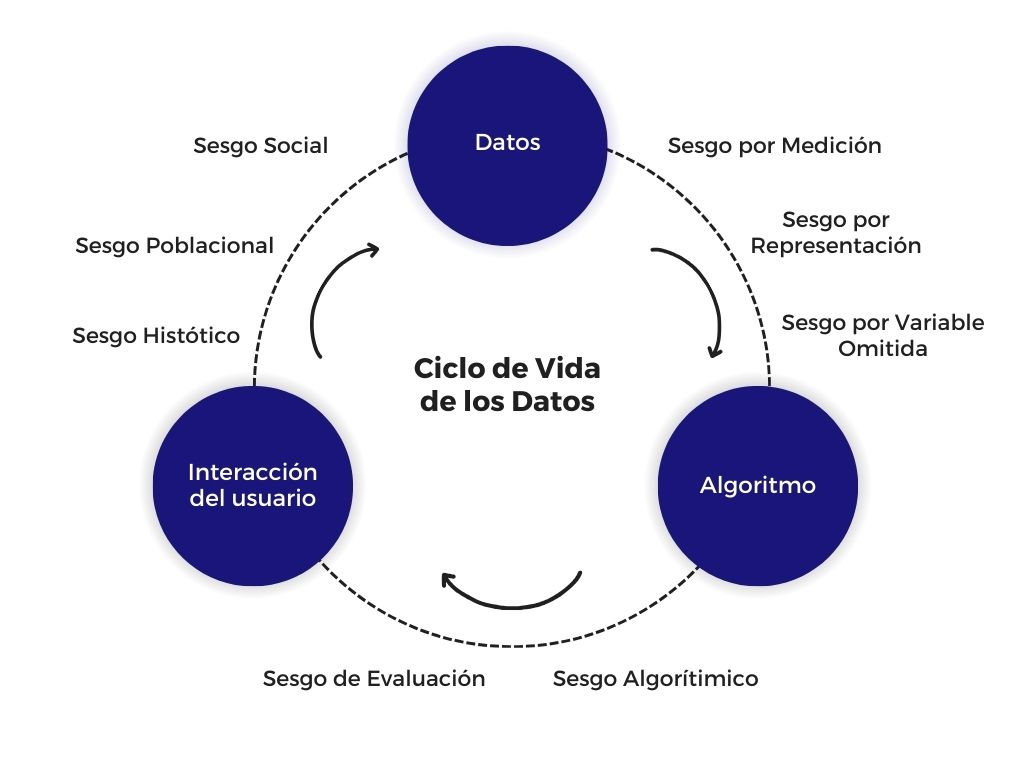
\includegraphics[width=0.7\textwidth]{Graphics/data_cycle.png}
        \end{center}
        \caption{Ejemplos de definiciones de sesgo ubicadas en el ciclo de vida de los datos.}
        \label{fig:cycle}
    \end{figure}
    

    \subsection{Sesgos de los datos al algoritmo}
    
    \begin{itemize}
        \item \textbf{Sesgo por medici\'on}: Este sesgo surge de como se eligen, utilizan y miden atributos particulares. Un ejemplo de esto se observa 
        en la herramienta de predicci\'on de riesgo de reincidencia COMPAS, donde detenciones anteriores y detenciones de amigos o familiares se utilizaron 
        como variables para medir peligrosidad.
        
        \item \textbf{Sesgo por variable omitida}: Este sesgo ocurre cuando una o m\'as variables importantes son excluidas del modelo. Decir algo mas
        
        \item \textbf{Sesgo por representaci\'on}: Este sesgo se produce de c\'omo se seleccionan las muestras de una poblaci\'on durante el proceso de
        recopilaci\'on de datos. Las muestras no representativas carecen de la diversidad de la poblaci\'on, con subgrupos faltantes y otras anomal\'ias.
    \end{itemize}
    
    \subsection{Sesgos del algoritmo al usuario}

    \begin{itemize}
        \item \textbf{Sesgo algor\'itmico}: El sesgo algor\'itmico se presenta cuando el sesgo no est\'a presente en los datos de entrada
        y se agrega puramente por el algoritmo. Las elecciones de dise\~no algor\'itmico, como el uso de ciertas funciones de optimizaci\'on, 
        regularizaciones, decisiones en la aplicaci\'on de modelos de regresi\'on en los datos en su totalidad o considerando subgrupos, y el uso
        general de estimadores estad\'isticamente sesgados en algoritmos, todos pueden contribuir a decisiones algor\'itmicas sesgadas que 
        afectan los resultados de los algoritmos. 
        
        \item \textbf{Sesgo por la interacci\'on del usuario}: El sesgo de interacci\'on del usuario no solo puede observarse en la web, sino que 
        tambi\'en puede ser producido por dos fuentes: la interfaz de usuario y cuando el propio usuario impone su comportamiento sesgado.
        
        \item \textbf{Sesgo de evaluaci\'on}: El sesgo de evaluci\'on ocurre durante la evaluaci\'on del modelo. Esto incluye el uso de m\'etricas
        inapropiadas y desproporcionadas para la evaluaci\'on del modelo. Un ejemplo de esto son las m\'etricas \textit{Adience} y \textit{IJB-A}, 
        que se utilizan en la evaluaci\'on de sistemas de reconocimiento facial que estaban sesgados hacia el color de la piel y el g\'enero.
    \end{itemize}
    
    \subsection{Sesgos del usuario a los datos}

    \begin{itemize}
        \item \textbf{Sesgo hist\'orico}: El sesgo hist\'orico es el sesgo y los problemas sociot\'ecnicos ya existentes en el mundo y puede 
        generarse desde el proceso de generaci\'on de datos incluso con un muestreo y selecci\'on de caracter\'isticas perfectos.

        \item \textbf{Sesgo poblacional}: El sesgo poblacional surge cuando las estad\'isticas, demograf\'ias, representantes y caracter\'isticas 
        de los usuarios son diferentes en la poblaci\'on de usuarios de la plataforma con respecto a la poblaci\'on objetivo original, creando datos no
        representativos. Un ejemplo de este tipo de sesgo puede surgir de las diferentes demograf\'ias de usuarios en las plataformas sociales, como las
        mujeres que son m\'as propensas a usar \textit{Pinterest}, \textit{Facebook}, \textit{Instagram}, mientras que los hombres son m\'as activos en 
        foros en l\'inea como \textit{Reddit} o \textit{X}.

        \item \textbf{Sesgo social}: El sesgo social se produce cuando las acciones de otros afectan el juicio de una persona. Un ejemplo de este tipo de 
        sesgo podr\'ia ser un caso en el que la persona quiere calificar o revisar un elemento con puntuaci\'on baja, pero al ser influenciada por otras
        calificaciones altas, cambia su puntuaci\'on a una calificaci\'on m\'as alta, pensando que quiz\'as esta siendo demasiado severa.
    \end{itemize}

\section{Detecci\'on y mitigaci\'on de sesgos}

Las definiciones de equidad en el contexto de los modelos de aprendizaje de m\'aquinas nos llevan 
a un panorama complejo y en constante evoluci\'on. A d\'ia de hoy, no existe una definici\'on \'unica y precisa
de lo que constituye la equidad en este \'ambito. La implementaci\'on de algoritmos en la toma de decisiones automatizada ha desatado 
debates acerca de c\'omo conceptualizar y medir tanto la equidad como la justicia. Estos conceptos no solo involucran consideraciones 
t\'ecnicas, sino que tambi\'en se ven influidos por matices culturales y dilemas \'eticos.

\subsection{Definiciones de equidad}
Las diversas perspectivas sobre la equidad pueden agruparse en dos categor\'ias principales: a nivel de Grupos y a nivel Individual. 
A continuaci\'on se presentan algunas de las definiciones de equidad m\'as relevantes a nivel de grupos:

\begin{itemize}
    \item \textbf{Demographic Parity}: Un algoritmo predictor $\hat{Y}$ satisface \textit{Demographic Parity}
    con respecto a un atributo $A$ con valores en el conjunto $\{0,1\}$ si se cumple $P(\hat{Y} | A = 0) = P(\hat{Y} | A = 1)$. 
    Esto significa que la probabilidad de un resultado positivo debería ser la misma sin importar si el individuo pertenece a
    un grupo protegido~\parencite{fairness_def}.

    \item \textbf{Equal Opportunity}: Un predictor binario $\hat{Y}$ satisface \textit{Equal Opportunity} con 
    respecto a un atributo $A$ y salida $Y$ si $P(\hat{Y} = 1 | A = 1, Y = 1) = P(\hat{Y} = 1 | A = 0, Y = 1)$. Esto significa
    que la probabilidad de que a una persona en la clase positiva le sea asignada un resultado positivo 
    deber\'ia ser igual para miembros tanto de grupos protegidos como no protegidos~\parencite{fairness_def}.

    \item \textbf{Equalized Odds}: Un predictor $\hat{Y}$ satisface \textit{Equalized Odds} con respecto a un atributo
    protegido $A$ y predicci\'on $Y$, si $P(\hat{Y} = 1 | A = 1, Y = y) = P(\hat{Y} = 1 | A = 0, Y = y)$, es decir,
    $\hat{Y}$ y $A$ son independientemente condicionales a $Y$. Esto significa que la probabilidad de que a una persona 
    en la clase positiva le sea asignada correctamente una predicci\'on positiva y la probabilidad de que a una persona en la 
    clase negativa le sea incorrectamente asignada una predicci\'on positiva deber\'ia se la misma para miembros de grupos 
    protegidos y no protegidos~\parencite{fairness_def}.
\end{itemize}

% Otros enfoques relevantes para tratar los sesgos a nivel individual son:

% \begin{itemize}
%     \item \textbf{Fairness Through Awareness}: Individuos con caracter\'isticas similares seg\'un alg\'un criterio 
%     definido deber\'ian obtener resultados parecidos \parencite{fair_awareness}.
%     \item \textbf{Fairness Through Unawareness}: Un algoritmo se considera imparcial cuando no basa sus decisiones en el 
%     atributo protegido \parencite{counterfactual}.
%     \item \textbf{Conterfactual fairness}: Una decisi\'on es considerada imparcial hacia un individuo cuando es la misma
%     tanto en la situaci\'on real como en una situaci\'on hipot\'etica donde el individuo pertenece a otro grupo \parencite{counterfactual}.
% \end{itemize}

\subsection{Mitigaci\'on de sesgos}

Los algoritmos destinados a la mitigaci\'on de sesgos se pueden clasificar esencialmente en m\'etodos de 
pre-procesamiento~\parencite{osti_10182459}, durante el procesamiento~\parencite{ml_in_admissions} y 
post-procesamiento~\parencite{compas}, seg\'un la fase del proceso de aprendizaje en que se realizen. Recientemente, 
han surgido nuevos m\'etodos llamados meta-algoritmos que ofrecen resultados interesantes en diversos escenarios.

Las estrategias de pre-procesamiento buscan la equidad al modificar la representaci\'on de los datos antes de aplicar un modelo de aprendizaje
autom\'atico. En este proceso se pueden aplicar diversas t\'ecnicas sobre los datos, como eliminar atributos protegidos y atributos correlacionados
con estos, o bien, modificar las etiquetas de algunos objetos en el datset~\parencite{preproc}. Una ventaja de estas t\'ecnicas es que son independientes
al modelo. Sin embargo, requieren ajustes de hiperpar\'ametros tanto propios como del modelo seleccionado para optimizar su desempe\~no.

Los m\'etodos aplicados durante el procesamiento, modifican los algoritmos de aprendizaje para eliminar la fuente de discriminaci\'on. Esto se 
logra mediante ajustes en la funci\'on objetivo o la aplicaci\'on de restricciones espec\'ificas~\parencite{donini2020empirical,zafar17a}. A pesar de 
que estas t\'ecnicas pueden ser altamente efectivas para la clase espec\'ifica de modelos para la cual fueron dise\~nadas, resulta dif\'icil, e 
incluso en ocasiones imposible, extenderlas a nuevas clases de modelos.

Las t\'ecnicas de post-procesamiento se implementan despu\'es de que el modelo ha sido entrenado, utilizando un conjunto de datos que no haya
participado en dicho proceso. Mediante este procesamiento, las clasificaciones generadas por el modelo se reasignan mediante una funci\'on 
espec\'ifica~\parencite{d_Alessandro_2017}.
Entre las t\'ecnicas de post-procesamiento, se incluyen aquellas que buscan identificar los atributos protegidos que afectan el resultado del 
modelo, y a partir de esto, ajustan la predicci\'on~\parencite{seymour2018bias}. La principal limitaci\'on radica en que ajustar la predicci\'on 
en esta fase es inherentemente sub\'optimo y puede resultar en un peor equilibrio entre eficacia y equidad.

Por \'ultimo, cabe destacar la relevancia de los meta-algoritmos, una categor\'ia de m\'etodos recientemente propuesta para problemas de 
mitigaci\'on de sesgos. Estos simplifican la tarea de mitigaci\'on de sesgos a una serie de problemas de clasificaci\'on, cada uno con 
un costo asociado a sus errores de predicci\'on~\parencite{agarwal2018reductions, agarwal2019fair}.
A diferencia de los m\'etodos operan durante el procesamiento, los meta-algoritmos son independientes al tipo de modelo utilizado en el 
clasificador base, solo dependen de la capacidad de este para ser reentrenado repetidamente. Las soluciones a estos problemas suelen generar
un clasificador randomizado.

\subsection{Anotaci\'on autom\'atica de atributos protegidos}


\section{Datasets en el tratamiento de sesgos}
    % \begin{itemize}
    %     \item empezar hablando de como los datasets ayudan a desarrollar y evaluar tecnicas de evaluacion y mitigacion de sesgos
    %     \item luego mencionar y decir algo de los datasets clasicos con datos tabulares
    %     \item luego empezar a hablar de datasets con datos no tabulares en general y decir que hay pocos y que son dificiles de conseguir 
    %     \item hablar luego de datasets interesantes que se pueden utilizar para esto (los estudiados)
    %     \item Decir algunos datos interesantes de cada uno
    % \end{itemize}

    Los datasets con atributos protegidos anotados juegan un papel fundamental en el desarrollo y evaluaci\'on de t\'ecnicas destinadas 
    a mitigar sesgos. Estos proporcionan la informaci\'on necesaria para la identificaci\'on, cuantificaci\'on y abordaje de sesgos, 
    permitiendo as\'i la creaci\'on y validaci\'on de t\'ecnicas dirigidas a mejorar la equidad y justicia en modelos de aprendizaje 
    autom\'atico. 
    Un dataset representativo y diverso es esencial para el desarrollo de estrategias eficaces que mitiguen sesgos en diversas aplicaciones. 
    Los datasets pueden categorizarse en dos grupos seg\'un la configuraci\'on de sus datos: 
    aquellos con datos tabulares\footnote{Est\'a organizado en forma de tabla, donde los datos se presentan en filas y columnas. Cada fila 
    representa una entrada individual, y cada columna es una caracter\'istica espec\'ifica con valores num\'ericos, categ\'oricos u otros.} 
    y aquellos con datos no tabulares\footnote{No sigue la estructura de una tabla tradicional, puede tener informaci\'on m\'as compleja, como 
    texto, im\'agenes o audio}.
    
    \subsection{Datasets con datos tabulares}
    Entre los datasets con estructura tabular m\'as relevantes utilizados para el an\'alisis y la evaluaci\'on de modelos destinados 
    a la mitigaci\'on de sesgos~\parencite{calmon2017optimized,wang2023mitigating,compas}, se incluyen:

    %#TODO deberia annadir una tabla tambien de tabulares?????
    \begin{itemize}
        \item \textbf{Adult}: Tambi\'en conocido como \textit{Census Income}, este dataset contiene 48842 registros de 
        datos sobre el censo de 1994 en Estados Unidos. Incluye 14 atributos, como edad, educaci\'on, estado civil,
        ocupaci\'on, raza, g\'enero, pa\'is de origen, horas de trabajo por semana, entre otros. Adem\'as para cada 
        persona dice si sus ingresos son mayores o menores a 50 mil d\'olares anuales.
        \item \textbf{Compas}: Este dataset contiene 18610 registros de los acusados del condado de Broward, Florida,
        indicando sus tiempos en la c\'arcel y prisi\'on, datos demogr\'aficos, antecedentes penales y puntuaciones 
        de riesgo, desde 2013 hasta 2014.
        \item \textbf{German Credit}: El dataset \textit{German Credit} contiene 1000 registros crediticios que incluyen atributos 
        como estado personal y g\'enero, puntaje crediticio, monto del cr\'edito, estado de vivienda, entre otros. Adem\'as cada 
        persona es clasificada como un riesgo crediticio bueno o malo, seg\'un el conjunto de atributos.
        \item \textbf{Communities and Crime}: Este dataset recopila informaci\'on de diversas comunidades en Estados Unidos, 
        relacionada con varios factores que pueden influir significativamente en algunos delitos comunes, como robos, asesinatos o 
        violaciones. Los datos incluyen informaci\'on sobre delitos obtenida de la encuesta \textit{LEMAS} de Estados Unidos en 1990 y 
        del \textit{Informe Unificado de Delitos del FBI} en 1995. Adem\'as, se incluyen datos demogr\'aficos y socioecon\'omicos del 
        censo de 1990.

    \end{itemize}

    \subsection{Datasets con datos no tabulares}
    Los datasets con datos no tabulares y atributos protegidos anotados, como im\'agenes, audio, texto y otros formatos complejos, 
    son considerablemente menos comunes que los datasets con datos tabulares. Esto se debe a la complejidad y el costo asociado a la 
    recopilaci\'on, etiquetado y mantenimientode datos no tabulares.

    Mientras que los datos tabulares son adecuados para problemas estructurados, los datos no tabulares permiten abordar tareas m\'as diversas, 
    como reconocimiento de im\'agenes, procesamiento de lenguaje natural, an\'alisis de audio y textos. Esto los convierte en un recurso muy importantes
    para el desarrollo y evaluaci\'on de t\'ecnicas de mitigaci\'on de sesgos en estos escenarios. En la tabla~\ref{table:datasets} 
    se presentan algunos ejemplos relevantes de datasets con datos no tabulares y atributos protegidos anotados de inter\'es para el 
    an\'alisis de sesgos.

    %#TODO Preguntar al profe que cree de esta tabla, yo la veo rara, tal vez por el tamanno. Tal vez sea mejor la info de la tabla integrarla a los parrafos que hablan otros datos
    %de los datasets. 

    \begin{table}[htpb]
        \centering
        \resizebox{\textwidth}{!}{
            \begin{tabular}{lp{0.34\textwidth}p{0.34\textwidth}p{0.34\textwidth}}
            \toprule
            \toprule
                \textbf{Dataset}     & \textbf{Twitter Gender}                          & \textbf{Md Gender Funpedia}                         & \textbf{Bias in Toxicity}       \\
                \toprule
                \toprule
                Tipo de datos        & Texto                                            & Texto                                               & Texto                           \\
                \midrule
                Atributos protegidos & Existencia o no de sesgo                         & G\'enero                                            & G\'enero, raza, religi\'on, orientaci\'on sexual y discapacidad  \\
                \midrule
                Idioma               & Espa\~nol                                        & Ingl\'es                                            & Ingl\'es                        \\
                \midrule
                Lenguaje             & Chitchat                                         & Formal                                              & Informal                        \\
                \midrule
                Tama\~no             & 1.9K                                             & 29.8K                                               & 1.9M                            \\
                \midrule
                Tipo de Ann.         & Poner Algo                                       & Preanotado autom\'aticamente y revisado manualmente & Manual                          \\
                \midrule
                Fuente de datos      & P\'aginas web que abordan los sesgos de g\'enero & Wikipedia                                           & Plataforma Civil Comments       \\
                \toprule
                \toprule
                \textbf{Dataset}     & \textbf{Fair Face}                               & \textbf{UTKFace}                                    & \textbf{MTGenEval}              \\
                \toprule
                \toprule
                Tipo de datos        & Im\'agenes                                       & Im\'agenes                                          & Texto                           \\
                \midrule
                Atributos protegidos & G\'enero, raza y edad                            & G\'enero, raza y edad                               & G\'enero                        \\
                \midrule
                Idioma               & -                                                & -                                                   & Ingl\'es, espa\~nol, ar\'abico, franc\'es, alem\'an, hind\'u, italiano, portugu\'es y ruso\\
                \midrule
                Lenguaje             & -                                                & -                                                   & Informal                        \\
                \midrule
                Tama\~no             & 108K                                             & 20K                                                 & 4K                              \\
                \midrule
                Tipo de Ann.         & Manual                                           & Semi-autom\'atica                                   & Manual                          \\
                \midrule
                Fuente de datos      &  Dataset YFCC-100M Flickr                        & Datasets MORPH y CACD y web                         & Wikipedia                       \\
                \bottomrule
                \bottomrule
            \end{tabular}}
        \caption{Datasets con datos no tabulares}
        \label{table:datasets}
    \end{table}
    
    El dataset \textit{Twitter Gender}\footnote{\url{https://www.kaggle.com/datasets/kevinmorgado/gender-bias-spanish}} est\'a conformado por 
    tweets en espa\~nol etiquetados con la categor\'ia de sesgado o no sesgado. Inicialmente el dataset no est\'a dividido en subconjuntos de 
    entrenamiento y prueba.

    El dataset \textit{Md Gender Funpedia}\footnote{\url{https://huggingface.co/datasets/md_gender_bias/viewer/funpedia}} contiene oraciones de 
    Wikipedia, reformuladas de una manera m\'as conversacional~\parencite{dinan2020multidimensional}. Se conservan \'unicamente las oraciones 
    vinculadas a biograf\'ias. Cada oraci\'on est\'a etiquetada con el g\'enero de quien se habla. Adem\'as est\'a dividido en subconjuntos de 
    entrenamiento, prueba y validaci\'on.
    %#TODO ver como hacer para que las urls no me queden tan largan en los pie de pagina
    El dataset \textit{Bias in Toxicity}\footnote{\url{https://www.kaggle.com/competitions/jigsaw-unintended-bias-in-toxicity-classification}}
    est\'a formado por comentarios, con gran cantidad de atributos protegidos anotados: male, female, white, asian, entre otros. Tambi\'en se 
    indica el nivel de toxicidad y toxicidad severa de cada comentario. Cada atributo es un valor entre $0$ y $1$ que indica la probabilidad de 
    que el comentario pertenezca a la clase correspondiente. Este dataset aporta tambi\'en los subconjuntos de entrenamiento y prueba, adem\'as 
    de otros subconjuntos relacionados con la anotaci\'on del mismo.  

    El dataset \textit{Fair Face}\footnote{\url{https://github.com/joojs/fairface}} contiene im\'agenes de rostros, con los atributos edad, 
    g\'enero y raza anotados. Est\'a balanceado respecto a la raza~\parencite{karkkainenfairface} e incluye los subconjuntos de entrenamiento y 
    validaci\'on.

    El dataset \textit{UTKFace}\footnote{\url{https://www.kaggle.com/datasets/jangedoo/utkface-new}} est\'a formado por im\'agenes de rostros, que 
    presentan una gran variaci\'on en la pose, expresi\'on facial, iluminaci\'on, oclusi\'on y resoluci\'on~\parencite{zhang2017age}. 
    Tiene anotados los atributos protegidos edad, g\'enero y raza. Presenta desbalance respecto estos atributos, con predominio de la raza 
    blanca y el g\'enero masculino. Inicialmente no se incluyen los subconjuntos de entrenamiento y prueba.

    El dataset \textit{MTGenEval}\footnote{\url{https://github.com/amazon-science/machine-translation-gender-eval}} contiene oraciones en 
    diferentes idiomas que se traducen mejor considerando el contexto inter-sentencial\footnote{Se refiere a la informaci\'on que se puede 
    inferir de la oraci\'on} y oraciones que se traducen mejor cuando se cambia una palabra o frase espec\'ifica. Incluye atributos protegidos 
    relacionados con el g\'enero, ejemplos de oraciones estereotipadas y antiestereotipadas. Se utiliza para entrenar y evaluar modelos de 
    traducci\'on autom\'atica, prestando especial atenci\'on a la equidad de g\'enero en dichas traducciones~\parencite{Currey2022}.

\section{Discusi\'on}

Los datasets presentados anteriormente constituyen un recurso valioso para apoyar el estudio, desarrollo y evaluaci\'on de t\'ecnicas de 
mitigaci\'on de sesgos en modelos de aprendizaje autom\'atico. Sin embargo, la principal limitante de estos es que ninguno ofrece 
informaci\'on sobre decisiones tomadas sobre los sujetos, como la decisi\'on de otorgar un pr\'estamo o la de contratar a una persona.

Esta limitaci\'on es significativa porque impide una evaluaci\'on completa de si las decisiones tomadas por los algoritmos basados 
en los datos son sesgadas o no. Por ejemplo, si un algoritmo se utiliza para tomar decisiones de contrataci\'on bas\'andose en datos
sobre solicitantes de empleo, incluyendo su g\'enero y raza, ser\'ia \'util conocer si a cada solicitante se le ofreci\'o 
un trabajo o no. Esta informaci\'on permitir\'ia evaluar si el algoritmo se inclina a ofrecer trabajos a personas con cierto g\'enero o raza
por encima de otras.

Por lo tanto, en el contexto de esta tesis, que tiene como objetivo el dise\~no y evaluaci\'on de un dataset de datos no tabulares
con atributos protegidos anotados, es importante considerar la inclusi\'on de informaci\'on sobre las decisiones tomadas sobre los sujetos.
El dataset de rese\~nas de pel\'iculas \emph{IMDb}\footnote{\url{https://www.kaggle.com/datasets/mantri7/imdb-movie-reviews-dataset}}
cumple con esta restricci\'on, ya que incluye el sentimiento presente en cada rese\~na, que puede considerarse como una decisi\'on de 
recomendaci\'on. Adem\'as si se realiza la anotaci\'on manual de los atributos g\'enero y raza para cada textp, se obtendr\'ia un dataset
que cumple con todas las restricciones planteadas en los Objetivos Generales.
\chapter{Descripci\'on del Corpus}\label{chapter:proposal}
En este cap\'itulo se propone una metodolog\'ia de anotaci\'on de prop\'osito general de atributos protegidos
en textos. 
AQUI HAY QUE HACER UN PARRAFITO DESCRIBIENDO TODO LO QUE SE VA A HACER EN ESTE CAPITULO Y COMO SE VA A ORGANIZAR

\section{Esquema de anotaci\'on}
%Hablar de que cada elemento a anotar es un texto, no una sola oracion.ok
%Hablar de cuales son los atributos protegidos que se anotaron. ok
%Hablar de los valores de cada atributo protegido y mas cosas relacionadas.
En el proceso de construcci\'on del corpus, cada elemento a anotar es un texto completo y no una oraci\'on individual. 
Este enfoque permite capturar el contexto completo en el que se producen las menciones a los atributos protegidos, 
lo cual es importante para poder realizar un an\'alisis m\'as profundo de (decir algo aqui como que es mejor asi para tratar los sesgos).

En este caso, los atributos protegidos que se van a anotar son el g\'enero y la raza.
Fueron seleccionados estos atributos no solo por su relevancia en diversas \'areas de estudio y aplicaci\'on, sino tambi\'en 
por la naturaleza de los textos que se van a anotar. Dado que las rese\~nas de pel\'iculas y series de televisi\'on
pueden contener un amplia gama de discusiones sobre actores, directores y personajes, es muy probable que se haga menci\'on a 
estos atributos.

Para el atributo g\'enero los valores a anotar son: "Male" para g\'enero masculino, "Female" para g\'enero femenino, 
"Male, Female" cuando se detectan ambos g\'eneros y "Null" en caso de no detectar ninguno.

En cuanto a la raza, los valores a anotar son: "White" para raza blanca, "Black" para raza negra, "Indian" para 
personas originarias de la India, "Arab" para personas de origen \'arabe, que incluye a pa\'ises del medio oriente y el norte de \'Africa.
Adem\'as se incorpora el valor "Latino" para personas de origen latinoamericano, "Native American" para personas originarias de 
los pueblos nativos de Am\'erica del Norte y "Asian" para personas asi\'aticas. Al igual que con el g\'enero, "Null" indica que no se detecta
ninguna raza en el texto. N\'otese que, en caso de ser necesario la anotaci\'on de la raza de un texto puede incluir m\'as de un valor.

\section{Proceso de anotaci\'on}

\subsection{Evaluaci\'on de la anotaci\'on}

\subsection{Directrices de anotaci\'on}
%Hablar que para anotar cierto atributo no hacer falta que el texto lo mencione explicitamente, sino que se puede inferir
%Ejemplo las entidades nombradas

\subsection{Herramientas de anotaci\'on}
%Describir los scripts que se hicieron para anotar, mezclar y todo eso


\section{Estad\'isticas del Corpus}

\section{Baselines}

\subsection{Detalles de implementaci\'on}


\chapter{An\'alisis Experimental}\label{chapter:implementation}
En este cap\'itulo, se presenta el marco experimental dise\~nado para comprobar la efectividad del modelo de anotaci\'on 
descrito en el Cap\'itulo~\ref{chapter:proposal}, y la calidad del corpus generado. Se describen las configuraciones y 
par\'ametros utilizadas en el proceso de validaci\'on y evaluaci\'on. Adem\'as, se muestran los resultados obtenidos y 
se realiza un an\'alisis de los mismos.

\section{Marco Experimental}\label{section:experimental_framework}
El marco experimental dise\~nado tiene como objetivo evaluar la validez de la propuesta desarrollada. Se plantea 
una experimentaci\'on que permite comprobar si la soluci\'on cumple con los requisitos y restricciones establecidos inicialmente.
Para ello, se proporcionan especificaciones detalladas acerca del corpus utilizado y los escenarios de evaluaci\'on desarrollados.
Adem\'as, se describen los hiperpar\'ametros utilizados y el hardware empleado para la experimentaci\'on.

\subsection{Escenarios de Evaluaci\'on}
La experimentaci\'on realizada se divide en dos escenarios. El primero de ellos se centra en analizar la concordancia alcanzada entre 
los anotadores humanos durante el proceso de construcci\'on del corpus. El segundo escenario, se orienta a utilizar el corpus 
desarrollado para entrenar y evaluar la eficacia de un modelo de clasificaci\'on de g\'enero y raza. Esto tiene como objetivo determinar
la capacidad de un anotador autom\'atico en replicar de manera confiable las anotaciones realizadas por los anotadores humanos. 

\subsubsection{Escenario I: Concordancia entre Anotadores}
Este escenario tiene como objetivo examinar la concordancia entre anotadores planteada en la 
secci\'on~\ref{subsection:annotation_evaluation}. El escenario busca obtener una estimaci\'on confiable de la dificultad de la 
tarea de anotaci\'on, as\'i como evaluar la calidad global de las anotaciones obtenidas. Esto se logra mediante la comparaci\'on
de las anotaciones realizadas de forma independiente por los dos anotadores no expertos, adem\'as de la comparaci\'on con la 
versi\'on final del corpus.

El an\'alisis de m\'etricas de concordancia inter-anotador permite determinar si las directrices propuestas en la 
secci\'on~\ref{section:annotation_guidelines} fueron adecuadas. Tambi\'en verifica si el proceso dise\~nado logra generar
anotaciones consistentes entre distintos anotadores. Una alta concordancia respalda la validez del proceso de anotaci\'on
planteado.

Adicionalmente, se quiere evaluar la calidad que tendr\'ia un anotador autom\'atico de prop\'osito general. Para esto, se 
emplea \emph{ChatGPT}~3.5 como anotador autom\'atico, y se comparan sus anotaciones con el corpus final.

\subsubsection{Escenario II: Evaluaci\'on de Baselines}
Este escenario tiene como objetivo evaluar los baselines dise\~nados en la secci\'on~\ref{section:baseline}, con el fin de 
validar su desempe\~no sobre el corpus desarrollado.

Para el obtener los \emph{embeddings} de los textos utilizados en el proceso de entrenamiento del \emph{baseline} 
de aprendizaje autom\'atico, se utilizaron cuatro modelos de \emph{BERT} que ofrece \emph{HuggingFace}.
Por tanto se tienen cuatro conjuntos de \emph{embeddings} diferentes para el entrenamiento de cada uno de 
los modelos estudiados. La Tabla~\ref{table:bert_models} muestra una comparaci\'on entre los modelos de \emph{BERT} utilizados.
De esta forma, se analiza el impacto de utilizar distintos modelos de \emph{BERT} para la representaci\'on 
sem\'antica de los textos sobre el desempe\~no de los \emph{baselines}. Los resultados obtenidos con cada 
combinaci\'on de modelo de \emph{BERT} y clasificador se reportan en la secci\'on~\ref{section:results}.

\begin{table}[htpb]
    \centering
    \resizebox{\textwidth}{!}{
        \begin{tabular}{lccc}
        \toprule
                \textbf{Modelo BERT} & \textbf{Par\'ametros} & \textbf{Dimensi\'on de Embeddings} & \textbf{Sensibilidad a May\'usculas}\\
                bert-base-uncased  & 110M & 768  & No\\
                bert-base-cased    & 110M & 768  & S\'i\\
                bert-large-uncased & 340M & 1024 & No\\
                bert-large-cased   & 340M & 1024 & S\'i\\
        \bottomrule
        \end{tabular}}
    \caption{Comparativa de modelos de \emph{BERT} utilizados.}
    \label{table:bert_models}
\end{table}

\subsubsection{M\'etricas de evaluaci\'on}
Las m\'etricas empleadas fueron macro precisi\'on, macro recobrado, macro puntuaci\'on F1 y 
macro exactitud. Estas fueron calculadas apoy\'andose en las siguientes variables: 

\begin{itemize}
    \item \textbf{Anotaciones Positivas Correctas (TP)}: N\'umero de instancias positivas correctamente clasificadas.
    \item \textbf{Anotaciones Positivas Incorrectas (FP)}: N\'umero de instancias negativas clasificadas como positivas.
    \item \textbf{Anotaciones Negativas Correctas (TN)}: N\'umero de instancias negativas correctamente clasificadas.
    \item \textbf{Anotaciones Negativas Incorrectas (FN)}: N\'umero de instancias positivas clasificadas como negativas.
\end{itemize}

Las versiones macro de las m\'etricas se calculan promediando cada valor obtenido de las siguientes ecuaciones:

\begin{align*}
    Precision_{attr} &= \frac{TP_{attr}}{TP_{attr} + FP_{attr}}\\
    Recobrado_{attr} &= \frac{TP_{attr}}{TP_{attr} + FN_{attr}}\\
    F1_{attr} &= 2 \cdot \frac{{Precision_{attr}} \cdot {Recobrado_{attr}}}{{Precision_{attr}} + {Recobrado_{attr}}}\\
    Exactitud_{multiclase} &= \frac{TP_{multiclase} + TN_{multiclase}}{TP_{multiclase} + TN_{multiclase} + FP_{multiclase} + FN_{multiclase}}\\
\end{align*}


\subsection{Corpus de Evaluaci\'on}
El corpus utilizado para la experimentaci\'on corresponde al conjunto de 150 textos con anotaciones de g\'enero y raza
generadas durante la construcci\'on del mismo, tal como se describe en la secci\'on~\ref{section:annotation_process}.

Espec\'ificamente, para el Escenario I se emplean las siguientes versiones del corpus:
\begin{itemize}
    \item Versi\'on 1: Conjunto de 150 textos con las anotaciones realizadas por el anotador 1.
    \item Versi\'on 2: Conjunto de 150 textos con las anotaciones realizadas por el anotador 2.
    \item Corpus Final: Versi\'on final del corpus de 150 textos, luego del proceso de mezcla y revisi\'on por parte 
    del anotador experto.
\end{itemize}

La comparaci\'on entre estas tres versiones del corpus permite estimar de manera realista la concordancia entre los anotadores 
no expertos y la concordancia de cada uno de ellos con la versi\'on final revisada. 

En el Escenario II, se emplea la versi\'on final del corpus tanto para entrenar y evaluar el \emph{baseline} de aprendizaje 
autom\'atico, como para evaluar el \emph{baseline} humano.

Para llevar a cabo estas evaluaciones, se emplea la 
metodolog\'ia \emph{K-fold cross-validation}. En este proceso, el modelo se entrena $K$ veces, utilizando 
$K-1$ particiones del corpus como conjunto de entrenamiento y la partici\'on restante como conjunto de evaluaci\'on.
Este enfoque enfoque permite obtener m\'etricas de rendimiento m\'as robustas y confiables, teniendo en cuenta 
la limitada cantidad de datos disponibles.

Para ambos \emph{baselines}, se elimina una fila del corpus. La raz\'on detr\'as de esto es que el atributo raza de dicha 
fila conten\'ia la \'unica instancia de la clase \emph{Native American} en el corpus. 
Esto genera conflictos durante el proceso de validaci\'on cruzada, ya que idealmente deber\'ian existir al menos dos 
instancias de cada clase en el corpus.

\subsection{Hiperpar\'ametros}
En el proceso de entrenamiento y evaluaci\'on de ambos \emph{baselines} el par\'ametro de la t\'ecnica de validaci\'on
cruzada se fija en $K=5$. 

\subsection{Hardware}
Los experimentos fueron ejecutados en un equipo con las siguientes propiedades: 4 n\'ucleos de CPU \emph{Intel(R) Core(TM)} i7-6700K
@ 4.00GHz de velocidad con 8 MB de cach\'e y 16 GB de RAM DDR4 a una velocidad de 3200MHz.

El sistema operativo utilizado fue \emph{Windows 10 Pro}, versi\'on 21H2 y con una arquitectura de 64 bits.

\section{Resultados}\label{section:results}
A continuaci\'on se muestran los resultados obtenidos a partir de realizar los experimentos de la forma descrita en la 
secci\'on~\ref{section:experimental_framework}.

La Tabla~\ref{table:agreement_humans} y la Tabla~\ref{table:agreement_gpt} muestran los resultados del \textbf{Escenario~I}.
Estas tablas resumen los resultados de las m\'etricas de concordancia calculadas entre las distintas
versiones del corpus y el anotador autom\'atico \emph{ChatGPT}~3.5, respectivamente. En ellas, se 
calcula para los conjuntos $C_{g\acute{e}nero}$, $C_{raza}$ y $C_{g\acute{e}nero, raza}$ definidos
en la secci\'on~\ref{subsection:annotation_evaluation} las m\'etricas: media, varianza y desviaci\'on
est\'andar. Adem\'as, se calcula el \emph{macro-agreement} definido en dicha secci\'on.

\begin{table}[htpb]
    \centering
    \resizebox{\textwidth}{!}{
        \begin{tabular}{llccc}
        \toprule
        \textbf{M\'etrica de concordancia} &&\textbf{Ver. 1 - Ver. 2} & \textbf{Ver. 1 - Final} & \textbf{Ver. 2 - Final} \\
        \midrule
        \midrule
        \multirow{3}{*}{G\'enero} & $\mu C_{g\acute{e}nero}$                & 0.873 & 0.917 & 0.943\\
        \cmidrule{2-5}
                                  & $\sigma C_{g\acute{e}nero}$             & 0.324 & 0.268 & 0.228\\
        \cmidrule{2-5}
                                  & $\sigma^2 C_{g\acute{e}nero}$           & 0.105 & 0.072 & 0.052\\
        \midrule\midrule
        \multirow{3}{*}{Raza}     & $\mu C_{raza}$                          & 0.898 & 0.917 & 0.981\\
        \cmidrule{2-5}
                                  & $\sigma C_{raza}$                       & 0.279 & 0.256 & 0.124\\
        \cmidrule{2-5}
                                  & $\sigma^2 C_{raza}$                     & 0.078 & 0.066 & 0.015\\
        \midrule\midrule
        \multirow{4}{*}{General}  & $\mu C_{g\acute{e}nero, raza}$          & 0.870 & 0.903 & 0.956\\
        \cmidrule{2-5}
                                  & $\sigma C_{g\acute{e}nero, raza}$       & 0.263 & 0.232 & 0.173\\
        \cmidrule{2-5}
                                  & $\sigma^2 C_{g\acute{e}nero, raza}$     & 0.069 & 0.054 & 0.030\\
        \cmidrule{2-5}
                                  & Macro Agr                               & 0.886 & 0.917 & 0.962\\
        \bottomrule
        \end{tabular}}
    \caption{Resumen de m\'etricas de concordancia entre las distintas versiones del corpus.}
    \label{table:agreement_humans}
\end{table}

\begin{table}[htpb]
    \centering
    \resizebox{0.75\textwidth}{!}{
        \begin{tabular}{llc}
        \toprule
        \textbf{M\'etrica de concordancia} &&\textbf{ChatGPT - Final} \\
        \midrule
        \midrule
        \multirow{3}{*}{G\'enero} & $\mu C_{g\acute{e}nero}$                & 0.350\\
        \cmidrule{2-3}
                                  & $\sigma C_{g\acute{e}nero}$             & 0.455\\
        \cmidrule{2-3}
                                  & $\sigma^2 C_{g\acute{e}nero}$           & 0.207\\
        \midrule\midrule
        \multirow{3}{*}{Raza}     & $\mu C_{raza}$                          & 0.371\\
        \cmidrule{2-3}
                                  & $\sigma C_{raza}$                       & 0.475\\
        \cmidrule{2-3}
                                  & $\sigma^2 C_{raza}$                     & 0.225\\
        \midrule\midrule
        \multirow{4}{*}{General}  & $\mu C_{g\acute{e}nero, raza}$          & 0.329\\
        \cmidrule{2-3}
                                  & $\sigma C_{g\acute{e}nero, raza}$       & 0.352\\
        \cmidrule{2-3}
                                  & $\sigma^2 C_{g\acute{e}nero, raza}$     & 0.124\\
        \cmidrule{2-3}
                                  & Macro Agr                               & 0.361\\
        \bottomrule
        \end{tabular}}
    \caption{Resumen de m\'etricas de concordancia entre \emph{ChatGPT} y corpus final.}
    \label{table:agreement_gpt}
\end{table}

En cuanto al \textbf{Escenario~II}, la Tabla~\ref{table:eval_baseline1_gender} y la Tabla~\ref{table:eval_baseline1_race}
muestran las m\'etricas alcanzadas por el \emph{baseline} de aprendizaje autom\'atico en la tarea de 
predicci\'on de los atribuitos g\'enero y raza respectivamente. Se presentan los resultados considerando 
diversas combinaciones entre los modelos de \emph{BERT} utilizados para obtener los \emph{embeddings} de los textos, y los
modelos de clasificaci\'on evaluados. 

Por otro lado, en la Tabla~\ref{table:eval_baseline2_gender} y la Tabla~\ref{table:eval_baseline2_race} se detallan
los resultados del \emph{baseline} humano en la misma tarea de predicci\'on de g\'enero y raza. 


\begin{table}[htpb]
    \centering
    \resizebox{\textwidth}{!}{
        \begin{tabular}{llcccc}
        \toprule
        \textbf{Combinaci\'on de Modelos} &&\textbf{Precisi\'on} & \textbf{Recobrado} & \textbf{F1} & \textbf{Exactitud}\\
        \midrule
        \midrule
        \multirow{4}{*}{bert-base-uncased}  & \emph{Logistic Regression}  & 0.740 & 0.788 & 0.757 & 0.366\\
        \cmidrule{2-6}
                                            & \emph{Random Forest}        & 0.695 & 0.816 & 0.744 & 0.308\\
        \cmidrule{2-6}
                                            & \emph{SVC}                  & 0.671 & 0.867 & 0.749 & 0.302\\
        \cmidrule{2-6}
                                            & \emph{MLP}                  & 0.733 & 0.788 & 0.753 & 0.375\\
        \midrule\midrule
        \multirow{4}{*}{bert-base-cased}    & \emph{Logistic Regression}  & 0.707 & 0.768 & 0.732 & 0.356\\
        \cmidrule{2-6}
                                            & \emph{Random Forest}        & 0.673 & 0.718 & 0.689 & 0.300\\
        \cmidrule{2-6}
                                            & \emph{SVC}                  & 0.621 & 1.000 & 0.764 & 0.257\\
        \cmidrule{2-6}
                                            & \emph{MLP}                  & 0.743 & 0.734 & 0.727 & 0.387\\
        \midrule\midrule
        \multirow{4}{*}{bert-large-uncased} & \emph{Logistic Regression}  & 0.707 & 0.787 & 0.741 & 0.366\\
        \cmidrule{2-6}
                                            & \emph{Random Forest}        & 0.684 & 0.771 & 0.719 & 0.343\\
        \cmidrule{2-6}
                                            & \emph{SVC}                  & 0.617 & 1.000 & 0.761 & 0.250\\
        \cmidrule{2-6}
                                            & \emph{MLP}                  & 0.695 & 0.751 & 0.718 & 0.404\\
        \midrule\midrule
        \multirow{4}{*}{bert-large-cased}   & \emph{Logistic Regression}  & 0.713 & 0.790 & 0.744 & 0.366\\
        \cmidrule{2-6}
                                            & \emph{Random Forest}        & 0.691 & 0.739 & 0.709 & 0.319\\
        \cmidrule{2-6}
                                            & \emph{SVC}                  & 0.639 & 0.848 & 0.722 & 0.275\\
        \cmidrule{2-6}
                                            & \emph{MLP}                  & 0.725 & 0.755 & 0.728 & 0.345\\
        \bottomrule
        \end{tabular}}
    \caption{Resumen de m\'etricas de evaluaci\'on del \emph{baseline} 1 en cuanto a la predicci\'on del atributo g\'enero.}
    \label{table:eval_baseline1_gender}
\end{table}

\begin{table}[htpb]
    \centering
    \resizebox{\textwidth}{!}{
        \begin{tabular}{llcccc}
        \toprule
        \textbf{Combinaci\'on de Modelos} &&\textbf{Precisi\'on} & \textbf{Recobrado} & \textbf{F1} & \textbf{Exactitud}\\
        \midrule
        \midrule
        \multirow{4}{*}{bert-base-uncased}  & \emph{Logistic Regression}  & 0.153 & 0.142 & 0.143 & 0.177\\
        \cmidrule{2-6}
                                            & \emph{Random Forest}        & 0.141 & 0.132 & 0.133 & 0.192\\
        \cmidrule{2-6}
                                            & \emph{SVC}                  & 0.098 & 0.165 & 0.123 & 0.132\\
        \cmidrule{2-6}
                                            & \emph{MLP}                  & 0.162 & 0.151 & 0.154 & 0.186\\
        \midrule\midrule
        \multirow{4}{*}{bert-base-cased}    & \emph{Logistic Regression}  & 0.158 & 0.147 & 0.148 & 0.179\\
        \cmidrule{2-6}
                                            & \emph{Random Forest}        & 0.114 & 0.136 & 0.124 & 0.151\\
        \cmidrule{2-6}
                                            & \emph{SVC}                  & 0.097 & 0.167 & 0.123 & 0.129\\
        \cmidrule{2-6}
                                            & \emph{MLP}                  & 0.181 & 0.188 & 0.177 & 0.205\\
        \midrule\midrule
        \multirow{4}{*}{bert-large-uncased} & \emph{Logistic Regression}  & 0.112 & 0.119 & 0.115 & 0.155\\
        \cmidrule{2-6}
                                            & \emph{Random Forest}        & 0.100 & 0.113 & 0.106 & 0.149\\
        \cmidrule{2-6}
                                            & \emph{SVC}                  & 0.097 & 0.167 & 0.123 & 0.129\\
        \cmidrule{2-6}
                                            & \emph{MLP}                  & 0.124 & 0.117 & 0.118 & 0.171\\
        \midrule\midrule
        \multirow{4}{*}{bert-large-cased}   & \emph{Logistic Regression}  & 0.124 & 0.138 & 0.129 & 0.188\\
        \cmidrule{2-6}
                                            & \emph{Random Forest}        & 0.110 & 0.123 & 0.116 & 0.151\\
        \cmidrule{2-6}
                                            & \emph{SVC}                  & 0.098 & 0.167 & 0.123 & 0.132\\
        \cmidrule{2-6}
                                            & \emph{MLP}                  & 0.119 & 0.112 & 0.111 & 0.170\\
        \bottomrule
        \end{tabular}}
    \caption{Resumen de m\'etricas de evaluaci\'on del \emph{baseline} 1 en cuanto a la predicci\'on del atributo raza.}
    \label{table:eval_baseline1_race}
\end{table}

\begin{table}[htpb]
    \centering
    \resizebox{0.75\textwidth}{!}{
        \begin{tabular}{lcccc}
        \toprule
        \textbf{Modelo} &\textbf{Precisi\'on} & \textbf{Recobrado} & \textbf{F1} & \textbf{Exactitud}\\
        \midrule
        \midrule
                       {Anotaci\'on 1}      & 0.937 & 1.000 & 0.967 & 0.872\\
                       {Anotaci\'on 2}      & 1.000 & 0.947 & 0.971 & 0.957\\
        \bottomrule
        \end{tabular}}
    \caption{Resumen de m\'etricas de evaluaci\'on del \emph{baseline} 2 en cuanto a la predicci\'on del atributo g\'enero.}
    \label{table:eval_baseline2_gender}
\end{table}

\begin{table}[htpb]
    \centering
    \resizebox{0.75\textwidth}{!}{
        \begin{tabular}{lcccc}
        \toprule
        \textbf{Modelo} &\textbf{Precisi\'on} & \textbf{Recobrado} & \textbf{F1} & \textbf{Exactitud}\\
        \midrule
        \midrule
                       {Anotaci\'on 1}      & 0.816 & 0.815 & 0.803 & 0.810\\
                       {Anotaci\'on 2}      & 0.900 & 0.878 & 0.886 & 0.959\\
        \bottomrule
        \end{tabular}}
    \caption{Resumen de m\'etricas de evaluaci\'on del \emph{baseline} 2 en cuanto a la predicci\'on del atributo raza.}
    \label{table:eval_baseline2_race}
\end{table}


\section{Discusi\'on}
Los resultados presentados en la Tabla~\ref{table:agreement_humans} indican un alto grado de concordancia entre las 
anotaciones realizadas por los distintos anotadores humanos.

Espec\'ificamente, la concordancia entre los anotadores no expertos (\textbf{Ver.~1 - Ver.~2}) es bastante alta. La
media de las concordancias por anotaci\'on supera \textbf{0.85} para g\'enero, raza y la uni\'on de ambas en una \'unica categor\'ia,
lo que indica un alto grado de concordancia promedio. Adem\'as, la varianza y desviaci\'on est\'andar est\'an por debajo de 
\textbf{0.11} y \textbf{0.33} respectivamente, lo que demuestra poca dispersi\'on en los valores de concordancia por texto. El
\emph{macro-agreement} de \textbf{0.886}, refuerza la consistencia en t\'erminos generales. Todo esto sugiere que las directrices 
de anotaci\'on fueron adecuadas y permitieron obtener anotaciones consistentes entre anotadores no expertos.

Al comparar las anotaciones de los no expertos con la versi\'on final (\textbf{Ver.~1 - Final} y \textbf{Ver.~2 - Final}), se
observa una mejor\'ia en las m\'etricas. La media supera \textbf{0.90} en todos los casos, la varianza y desviaci\'on est\'andar
disminuyen por debajo de \textbf{0.08} y \textbf{0.28} respectivamente, y el \emph{macro-agreement} aumenta a \textbf{0.917} y 
\textbf{0.962}. Esto indica que la revisi\'on por el experto incrementa significativamente la calidad y consistencia de las 
anotaciones.

Los resultados de la Tabla~\ref{table:agreement_gpt} muestran m\'etricas de concordancia significativamente menores entre 
el anotador autom\'atico \emph{ChatGPT} y el corpus final. La media se encuentra por debajo de \textbf{0.38} en todos los casos,
indicando un bajo grado de coincidencia promedio. Adem\'as, la varianza supera \textbf{0.20} en los casos de g\'enero y raza, y 
\textbf{0.12} en la uni\'on. La desviaci\'on est\'andar supera \textbf{0.35} en todos los casos. Todo esto indica una alta 
dispersi\'on en los valores de concordancia por texto respecto a los obtenidos por los anotadores humanos. El 
\emph{macro-agreement} de apenas \textbf{0.361} evidencia la falta de consistencia del anotador autom\'atico. En conjunto, estas
m\'etricas proveen evidencia de que un anotador autom\'atico de prop\'osito general como \emph{ChatGPT} no es capaz de replicar
de manera confiable las anotaciones realizadas por los anotadores humanos.  

Analizando los resultados mostrados en la Tabla~\ref{table:eval_baseline1_gender} para la predicci\'on de g\'enero con el 
\emph{baseline} de aprendizaje autom\'atico se observa que la exactitud alcanza valores hasta de \textbf{0.404}, 
evidenciando una capacidad moderada del clasificador para acertar en la predicci\'on de g\'enero. La precisi\'on se 
mantuvo en un rango entre \textbf{0.617} y \textbf{0.743} para todos los modelos, lo cual sugiere que los modelos no
clasifican demasiados falsos positivos. Las puntuaciones de recobrado fueron en general altas, superando \textbf{0.718}
en la mayor\'ia de los casos. Esto indica que los modelos en general clasifican bien las intancias positivas. Luego, las 
puntuaciones F1 se mantuvieron en un rango entre \textbf{0.689} y \textbf{0.764}, lo que indica que los modelos logran
un balance bastante aceptable entre precisi\'on y recobrado.

En contraste, los resultados para la predicci\'on de raza (Tabla~\ref{table:eval_baseline1_race}) con el 
\emph{baseline} de aprendizaje autom\'atico muestran m\'etricas considerablemente m\'as bajas. Tanto la 
precisi\'on como el recobrado de los modelos se mantuvieron por debajo de \textbf{0.190}, y en consecuencia 
las puntuaciones F1 no superan \textbf{0.180}. Todo esto indica de manera consistente que los modelos no 
logran clasificar correctamente las instancias positivas. Los valores para la exactitud no superan el puntanje 
de \textbf{0.205}. 

Estas diferencias tan marcadas en las m\'etricas de g\'enero y raza sugieren que predecir autom\'aticamente la 
raza a partir de texto presenta un desaf\'io significativamente mayor en comparaci\'on con la predicci\'on de 
g\'enero. 

Las m\'etricas obtenidas para el \emph{baseline} humano, mostradas en las 
Tablas~\ref{table:eval_baseline2_gender} y~\ref{table:eval_baseline2_race}, indican un desempe\~no muy 
superior al de los modelos de aprendizaje autom\'atico. 

Para la tarea de g\'enero (Tabla~\ref{table:eval_baseline2_gender}), la precisi\'on, recobrado, 
puntuaci\'on F1 y exactitud superan \textbf{0.870} para ambos anotadores. Lo que sugiere un 
rendimiento muy consistente y preciso en la clasificaci\'on tanto de instancias positivas, 
como de instancias negativas. En general se observa un desempe\~no superior del 
\emph{baseline} humano en comparaci\'on com el \emph{baseline} de aprendizaje autom\'atico en 
esta tarea.

Del mismo modo, para la predicci\'on de la raza, se obtienen valores de precisi\'on, recobrado,
puntuaci\'on F1 y exactitud muy prometedores para ambos anotadores. La precisi\'on y 
recobrado alcanzada por los anotadores superan \textbf{0.810}, y la puntuaci\'on F1 estuvo 
por encima de \textbf{0.80}. La exactitud tambi\'en fue muy alta, con valores de \textbf{0.810}
y \textbf{0.959}, evidenciando la gran habilidad de los humanos para replicar las anotaciones
de raza presentes en el corpus.

A pesar de que el \emph{baseline} humano logra m\'etricas de evaluaci\'on muy altas en ambas 
tareas, se aprecia cierto aumento en la dificultad de la tarea de predicci\'on de raza. Si bien 
los resultados alcanzados en la predicci\'on de la raza son muy buenos, su disminuci\'on 
comparados con los obtenidos en la predicci\'on de g\'enero sugiere que incluso para los humanos, 
no es una tarea trivial inferir la raza a partir de texto.

\backmatter

\begin{conclusions}
    Conclusiones
\end{conclusions}

\begin{recomendations}
    Recomendaciones
\end{recomendations}

\printbibliography[heading=bibintoc]


\end{document}